\documentclass[a4paper] {report}
%\usepackage {suthesis} % stanford thesis template
\usepackage {tikz}
\usepackage {enumerate}
\usepackage {graphicx}
\usepackage {color}
\usepackage {amsmath}
\usepackage {fontspec}
\usepackage{amsfonts} % uppercase math alphabet
\usepackage{booktabs}
\usepackage{amsmath} % for less equal and greater equal
\usepackage{amssymb} % for less equal and greater equal

\newcommand{\R}{\mathbb{R}}

\begin {document}

% Title
\title {Application of BERT in GMAT Exam Bank}
\author {Shark Deng}
\iffalse
\principaladviser {Pinghong Deng}  % suthesis
\firstreader {Pinghong Deng}
\secondreader {Pinghong Deng}
\thirdreader {Pinghong Deng}
\fi


% Preface
\iffalse
\beforepreface %suthesis
\input preface.tex
\input ack.tex
\afterpreface
\fi

% Ordered List
\begin {enumerate}
	\item bert
	\item attention is all you need
	\item stanford dissertation
\end {enumerate}

\begin {enumerate} [a)]
	\item banana
	\item apple
	\item strawberry
\end {enumerate}

% Unordered List
\begin {itemize}
	\item Moon
	\item Earth
\end {itemize}


% equation
\begin {equation} % with one line and number
	f(x) = 6*x+8
\end {equation}
$f(x) = 8*x^2$ % within one line
$$f(x) = 1/x$$  % with one line and without number


% insert image
\begin {figure}
	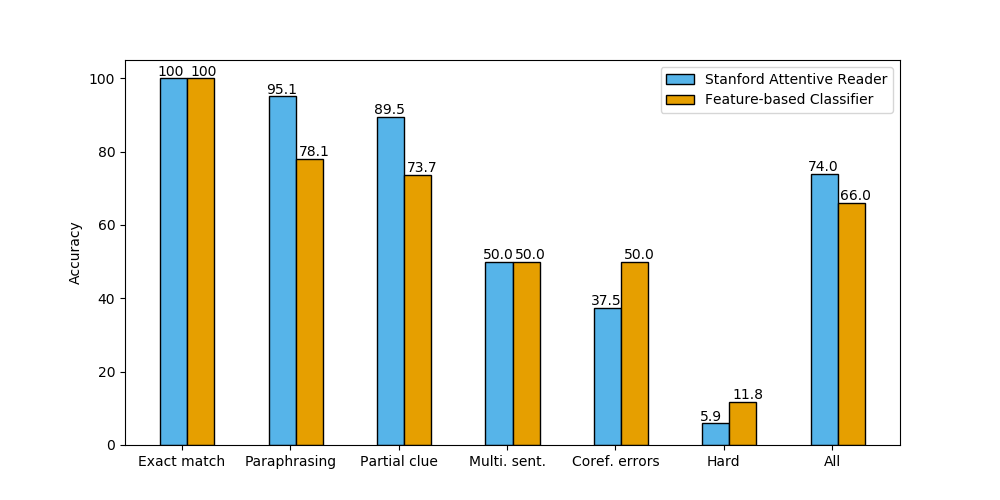
\includegraphics [width=1.77in] {../20190117/img/cnn_analysis.png}
\end {figure}


% typeset
\begin {flushright}
	To my parents, for their unconditional love
\end {flushright}

\begin {flushleft}
	Hello, my friends
\end {flushleft}

\newpage
\begin {flushright}
	hello
\end {flushright}


% word style
\textbf {BERT} 	\par		% bold

\emph {Italic}	\par		% italic

\underline {underline} \par	% underline

{\color {red} This word is red } \par

\textrm{Roman Family} \par
{\rmfamily Roman Family - Declaration Command} \par

\textsf{Sans Serif Family} \par
{\sffamily Sans Serif Family - Declaration Command} \par

\texttt{Typewriter Family} \par
{\ttfamily{Tywriter Family - Declaration Command} \par


{\tiny Hello} \\
{\scriptsize Hello} \\
{\small Hello}\\
{\normalsize Hello}\\
{\large Hello}\\
{\Large Hello}\\
{\LARGE Hello}\\
{\huge Hello}\\
{\Huge Hello}\\

% customized font
\newcommand{\myfont} {\textit{\textbf{\textsf {Fancy Text}}}}
\myfont


% Contents
\tableofcontents
\section {Section1}
Contents of Section 1
	\subsection {Easy is good}
Contents of subsection

% set







\begin{table}[h]
\begin{tabular}{c|c}
\toprule
Sepcial character & \alpha \quad \beta \quad \gamma \quad \delta \quad \epsilon \quad \varepsilon \quad \zeta \quad \eta \quad \theta \quad \iota \quad  \kappa \quad \lambda \quad \mu \quad \xi \quad \pi \quad \rho \quad \sigma \quad \tau \quad \upsilon \quad \phi \quad \chi \quad \psi \quad \omega \\
\hline
Set & $\subset$ \quad $\subseteq$ \quad $\in$ \quad $\cap$ \quad $\cup$ \quad $\mid$ \quad $\notin$ \\
\hline
Math alphabet & $\R$ \\
\hline
Equation & \le \quad \ge \quad $\leqslant$ \quad $\geqslant$ \\
Space & \qquad \quad a\ b a\;b a\,b ab a\!b \\
\bottomrule
\end{tabular}
\end{table}



























% font


\end {document}










